% =============================================================================
% SART method figure (standalone).
%
% Three iconic panels arranged left-to-right:
%   Step 1 (Score)   — gradient signatures A(s), R(s) -> ShortcutScore S(s)
%   Step 2 (Correct, NOVEL) — w(s) reweight + conflict-only PCGrad surgery
%   Step 3 (Apply)   — the corrected gradient enters the SGD/Adam update
%
% Built per the tikz-method-figure skill recipe: dashed panel boundaries,
% compound 2-line titles above, title-row inter-panel arrows, no math symbols
% inside the diagram beyond the small per-stage hyperparameter labels.
%
% Compile: pdflatex -interaction=nonstopmode sart_method_figure.tex
% Output:  sart_method_figure.pdf  (referenced from 3_overview.tex)
% =============================================================================
\documentclass[border=4pt]{standalone}
\usepackage{tikz}
\usepackage{amsmath,amssymb}
\usetikzlibrary{arrows.meta,positioning,shapes.geometric,shapes.symbols,decorations.pathreplacing,calc}

\begin{document}
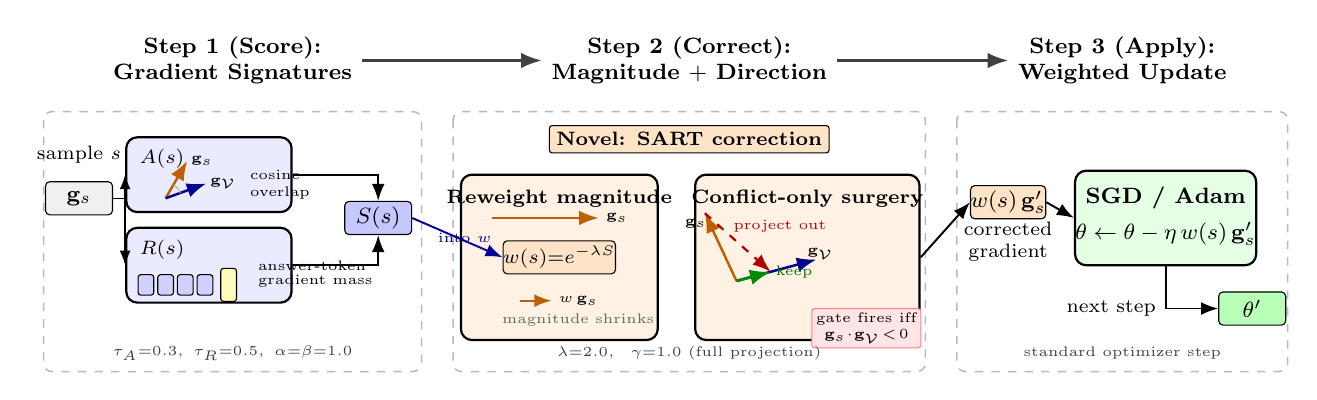
\begin{tikzpicture}[
  >=Latex,
  font=\small,
  title/.style       ={font=\footnotesize\bfseries, align=center},
  panelbox/.style    ={dashed, draw=gray!55, line width=0.55pt,
                       rounded corners=3pt},
  chip/.style        ={draw, rounded corners=1.5pt, minimum width=0.55cm,
                       minimum height=0.30cm, inner sep=0pt},
  scorechip/.style   ={chip, fill=blue!22, minimum width=0.85cm,
                       minimum height=0.42cm, font=\footnotesize},
  novelchip/.style   ={chip, fill=orange!22, minimum width=0.85cm,
                       minimum height=0.42cm, font=\footnotesize},
  graychip/.style    ={chip, fill=gray!18, minimum width=0.85cm,
                       minimum height=0.42cm, font=\footnotesize},
  ansbar/.style      ={draw, rounded corners=1pt, fill=yellow!28,
                       minimum width=0.20cm, minimum height=0.26cm,
                       inner sep=0pt, font=\tiny},
  reasonbar/.style   ={draw, rounded corners=1pt, fill=blue!18,
                       minimum width=0.20cm, minimum height=0.26cm,
                       inner sep=0pt, font=\tiny},
  databox/.style     ={draw, thick, rounded corners=4pt, fill=blue!8,
                       inner sep=4pt},
  novelbox/.style    ={draw, thick, rounded corners=4pt, fill=orange!10,
                       inner sep=4pt},
  applybox/.style    ={draw, thick, rounded corners=4pt, fill=green!10,
                       inner sep=4pt},
  novelflag/.style   ={draw, rounded corners=1pt, fill=orange!22,
                       font=\scriptsize\bfseries, inner sep=2.5pt, align=center},
  hyptag/.style      ={font=\tiny, align=center, text=black!75},
  flow/.style        ={->, thick, line width=0.7pt},
  thinflow/.style    ={->, thin, line width=0.5pt},
  stagearrow/.style  ={->, line width=1.0pt, draw=black!75},
  surgerykeep/.style ={->, line width=1.0pt, draw=green!55!black},
  surgerydrop/.style ={->, dashed, line width=0.8pt, draw=red!70!black},
  gvarrow/.style     ={->, line width=0.9pt, draw=blue!55!black},
  gsarrow/.style     ={->, line width=0.9pt, draw=orange!75!black},
]

% =====================================================================
% Panel 1: Score gradient signatures
% Boundary x-range: (-2.40, 2.40), center 0.00
% =====================================================================
\node[title] (T1) at (0.00, 2.30) {Step 1 (Score):\\Gradient Signatures};
\draw[panelbox] (-2.40, 1.65) rectangle (2.40, -1.65);

% Input: a sample's gradient g_s
\node[font=\scriptsize, align=center] (gsLabel) at (-1.95, 1.10) {sample $s$};
\node[chip, fill=gray!12, minimum width=0.85cm, minimum height=0.42cm, font=\footnotesize] (gsIn) at (-1.95, 0.55) {$\mathbf{g}_s$};

% Sub-icon A(s): cosine alignment with g_V
\node[databox, minimum width=2.10cm, minimum height=0.95cm] (boxA) at (-0.30, 0.85) {};
\node[font=\scriptsize\bfseries, anchor=north west] at (-1.30, 1.30) {$A(s)$};
% two arrows representing g_s and g_V at an angle (alignment / cosine)
\coordinate (origA) at (-0.85, 0.55);
\draw[gsarrow] (origA) -- ++(60:0.55) node[right, font=\tiny, inner sep=1pt] {$\mathbf{g}_s$};
\draw[gvarrow] (origA) -- ++(20:0.55) node[right, font=\tiny, inner sep=1pt] {$\mathbf{g}_{\mathcal V}$};
\draw[draw=gray!60, thin] (origA) ++(20:0.20) arc (20:60:0.20);
\node[font=\tiny, anchor=west] at (0.10, 0.85) {cosine};
\node[font=\tiny, anchor=west] at (0.10, 0.62) {overlap};

% Sub-icon R(s): answer-token concentration
\node[databox, minimum width=2.10cm, minimum height=0.95cm] (boxR) at (-0.30, -0.30) {};
\node[font=\scriptsize\bfseries, anchor=north west] at (-1.30, 0.15) {$R(s)$};
% token row with answer highlighted
\node[reasonbar] at (-1.10, -0.55) {};
\node[reasonbar] at (-0.85, -0.55) {};
\node[reasonbar] at (-0.60, -0.55) {};
\node[reasonbar] at (-0.35, -0.55) {};
\node[ansbar, minimum height=0.42cm] (ansbar) at (-0.05, -0.55) {};
\node[font=\tiny, anchor=west] at (0.20, -0.30) {answer-token};
\node[font=\tiny, anchor=west] at (0.20, -0.50) {gradient mass};

% S(s) output chip on the right
\node[scorechip] (Sout) at (1.85, 0.30) {$S(s)$};

% Arrows: g_s into both sub-icons
\draw[thinflow] (gsIn.east) -| ($(boxA.west)+(0,0)$);
\draw[thinflow] (gsIn.east) -| ($(boxR.west)+(0,0)$);
% Sub-icons combine into S(s)
\draw[flow] (boxA.east) -| ($(Sout.north)+(0,0)$);
\draw[flow] (boxR.east) -| ($(Sout.south)+(0,0)$);

% Hyperparameter footer (bottom row)
\node[hyptag] at (0.00, -1.42) {$\tau_A{=}0.3,\ \tau_R{=}0.5,\ \alpha{=}\beta{=}1.0$};

% =====================================================================
% Panel 2: Correct magnitude + direction (NOVEL)
% Boundary x-range: (2.80, 8.80), center 5.80
% =====================================================================
\node[title] (T2) at (5.80, 2.30) {Step 2 (Correct):\\Magnitude $+$ Direction};
\draw[panelbox] (2.80, 1.65) rectangle (8.80, -1.65);
\node[novelflag] at (5.80, 1.30) {Novel: SART correction};

% --- Sub-panel 2a: magnitude reweight (left half) ---
\node[novelbox, minimum width=2.50cm, minimum height=2.10cm] (boxRW) at (4.15, -0.20) {};
\node[font=\scriptsize\bfseries, anchor=north] at (4.15, 0.78) {Reweight magnitude};
% input g_s arrow (long)
\draw[gsarrow] (3.30, 0.30) -- (4.65, 0.30) node[right=-1pt, font=\tiny] {$\mathbf{g}_s$};
% w(s) chip (the multiplier)
\node[novelchip, font=\scriptsize] (wchip) at (4.15, -0.20) {$w(s){=}e^{-\lambda S}$};
% output: shorter arrow (downweighted) — placed below w(s) chip
\draw[gsarrow, line width=0.7pt] (3.65, -0.75) -- (4.05, -0.75) node[right=-1pt, font=\tiny] {$w\,\mathbf{g}_s$};
\node[font=\tiny, anchor=west, text=black!60] at (3.30, -1.00) {magnitude shrinks};

% --- Sub-panel 2b: direction surgery (right half) ---
\node[novelbox, minimum width=2.85cm, minimum height=2.10cm] (boxSurg) at (7.30, -0.20) {};
\node[font=\scriptsize\bfseries, anchor=north] at (7.30, 0.78) {Conflict-only surgery};
% Coordinate frame for the surgery diagram
\coordinate (surgOrig) at (6.40, -0.50);
% g_V (target direction)
\draw[gvarrow] (surgOrig) -- ++(15:1.05) coordinate (gvTip);
\node[font=\tiny, anchor=south west, inner sep=1pt] at ($(surgOrig)!0.85!(gvTip)$) {$\mathbf{g}_{\mathcal V}$};
% g_s (anti-aligned, obtuse angle from g_V)
\draw[gsarrow] (surgOrig) -- ++(115:0.95) coordinate (gsTip);
\node[font=\tiny, anchor=east, inner sep=1pt] at ($(surgOrig)!0.85!(gsTip)$) {$\mathbf{g}_s$};
% decompose g_s: keep parallel-to-g_V component (solid green) + drop perpendicular conflicting (dashed red)
% projection of g_s on g_V is small/negative — conceptually:
%   keep arrow runs along +g_V direction with small magnitude (or zero), but visualize the kept axis
%   drop arrow is the conflicting component (the part anti-aligned with g_V)
\draw[surgerykeep] (surgOrig) -- ++(15:0.45) node[right=-2pt, font=\tiny, text=green!45!black] {keep};
\draw[surgerydrop] (gsTip) -- ($(surgOrig) + (15:0.45)$);
\node[font=\tiny, text=red!70!black] at (6.95, 0.20) {project out};
% gate condition badge
\node[font=\tiny, align=center, draw=red!50, fill=red!10, rounded corners=1pt,
      inner sep=1.5pt] (gate) at (8.05, -1.10) {gate fires iff\\$\mathbf{g}_s\!\cdot\!\mathbf{g}_{\mathcal V} \!<\! 0$};

% Hyperparameter footer (bottom row)
\node[hyptag] at (5.80, -1.42) {$\lambda{=}2.0,\ \ \gamma{=}1.0$ (full projection)};

% =====================================================================
% Panel 3: Apply correction
% Boundary x-range: (9.20, 13.40), center 11.30
% =====================================================================
\node[title] (T3) at (11.30, 2.30) {Step 3 (Apply):\\Weighted Update};
\draw[panelbox] (9.20, 1.65) rectangle (13.40, -1.65);

% Input: corrected gradient
\node[novelchip, font=\footnotesize] (gprime) at (9.85, 0.50) {$w(s)\,\mathbf{g}'_s$};
\node[font=\scriptsize, align=center] at (9.85, 0.00) {corrected\\gradient};

% Update box
\node[applybox, minimum width=2.30cm, minimum height=1.20cm] (upd) at (11.85, 0.30) {};
\node[font=\footnotesize\bfseries] at (11.85, 0.55) {SGD / Adam};
\node[font=\footnotesize] at (11.85, 0.10) {$\theta \leftarrow \theta - \eta\, w(s)\,\mathbf{g}'_s$};

% Output: updated theta
\node[chip, fill=green!28, minimum width=0.85cm, minimum height=0.42cm, font=\footnotesize] (thetaOut) at (12.95, -0.85) {$\theta'$};
\node[font=\scriptsize, anchor=east] at (11.85, -0.85) {next step};

\draw[flow] (gprime.east) -- (upd.west);
\draw[flow] (upd.south) |- (thetaOut.west);

% Hyperparameter footer (note: total epochs = 50, warmup = max(5, epochs/6))
\node[hyptag] at (11.30, -1.42) {standard optimizer step};

% =====================================================================
% Title-row inter-panel arrows (above all boundary tops)
% =====================================================================
\draw[stagearrow] (T1.east) -- (T2.west);
\draw[stagearrow] (T2.east) -- (T3.west);

% =====================================================================
% Inter-panel content flow: S(s) -> reweight; (g_s, g_V) -> surgery; out -> apply
% =====================================================================
% S(s) chip flows into reweight w(s)
\draw[flow, draw=blue!60!black] (Sout.east) -- (wchip.west);
\node[font=\tiny, anchor=south, text=blue!55!black] at (2.95, -0.13) {into $w$};

% Apply panel input from surgery output: surgery -> corrected gradient chip
\draw[flow] (boxSurg.east) -- (gprime.west);

\end{tikzpicture}
\end{document}
